\documentclass{standalone}
\usepackage[dvipsnames,svgnames,x11names]{xcolor}
\usepackage{tikz}
\usepackage{pgfplots}
\pgfplotsset{compat = 1.12}
\usepackage{../thesismath}
\begin{document}
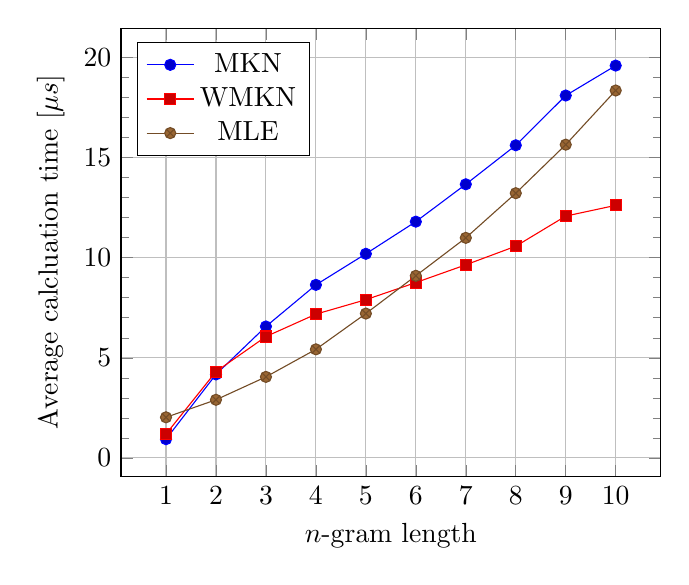
\begin{tikzpicture}[baseline]

\begin{axis}[
  xlabel = {$n$-gram length},
  xtick = {1, ..., 10},
  ylabel = {Average calcluation time [${\mu}s$]},
  minor y tick num = 4,
  grid = major,
  legend entries = {{MKN}, {WMKN}, {MLE}},
  legend pos = north west,
]

% MKN
\addplot table {
  n   us
  % sampled at N = 1000
  1    0.936
  2    4.171
  3    6.565
  4    8.643
  5   10.194
  6   11.800
  7   13.666
  8   15.614
  9   18.099
  10  19.594
};

% WMKN
\addplot table {
  n   us
  % sampled at N = 1000
  1    1.192
  2    4.311
  3    6.060
  4    7.180
  5    7.902
  6    8.758
  7    9.644
  8   10.573
  9   12.078
  10  12.614
};

% MKN
\addplot table {
  n   us
  % sampled at N = 1000
  1    2.028
  2    2.903
  3    4.047
  4    5.423
  5    7.210
  6    9.096
  7   10.991
  8   13.221
  9   15.645
  10  18.350
};

\end{axis}

\end{tikzpicture}
\end{document}
